\section{Introduction}
Video playback is supported in most of today's typical mobile devices. A recent study shows 20\% people watch videos on their mobile devices\cite{webbusinessinsider}.

Despite its popularity, several issues of mobile video playback remain unaddressed. Firstly, because its heavy processing requirement, High Definition (HD) video playback is not supported on many mobile devices. Secondly, video playback is energy demanding, and the fast pace discharge of battery makes the mobile devices ununsable quickly. 

The screen on mobile devices is usually not large, despite its high resolution. Pinch zoom and pan gestures have been widely adopted to help users to view photos, maps and web pages. Recent research indicates zoom and pan are helpful for users when watching videos\cite{Khiem:2011:TUU:2072298.2071917}. However, the examination of existing mobile video players on iPhone and Android platforms tell us many of them do not support zoom and pan. And for those supporting these gestures, they simply scale the video up.

When a video is scaled up, only part of the video scene are displayed. The visible part is referred as Region-of-Interest (ROI). The simple scale and display approach for video playback is inefficient since the entire video scene is decoded but only part of it is displayed. This observation presents an opportunity to achieve more efficient video playback on mobile devices. 

We propose a software approach named selective decoding that improves the efficiency of zoomable video playback. As its name suggests, this approach decodes video selectively based on the ROI captured from user interactions. With the improved efficiency, it is hoped this approach can help to address the two issues mentioned previously.

Our work is based on MPEG4 Part 2 Simple Profile (SP) codec, however this approach should be applicable for other Discrete Cosine Transform (DCT) based video codec. We focus our work on the decoder side of the codec in the local playback context, but the principles and techniques could be extended to encoder and video playback in network streaming context. A typical MPEG4 SP decoder is illustrated as below,
\begin{figure}
\centering
%\vspace{2.5cm}
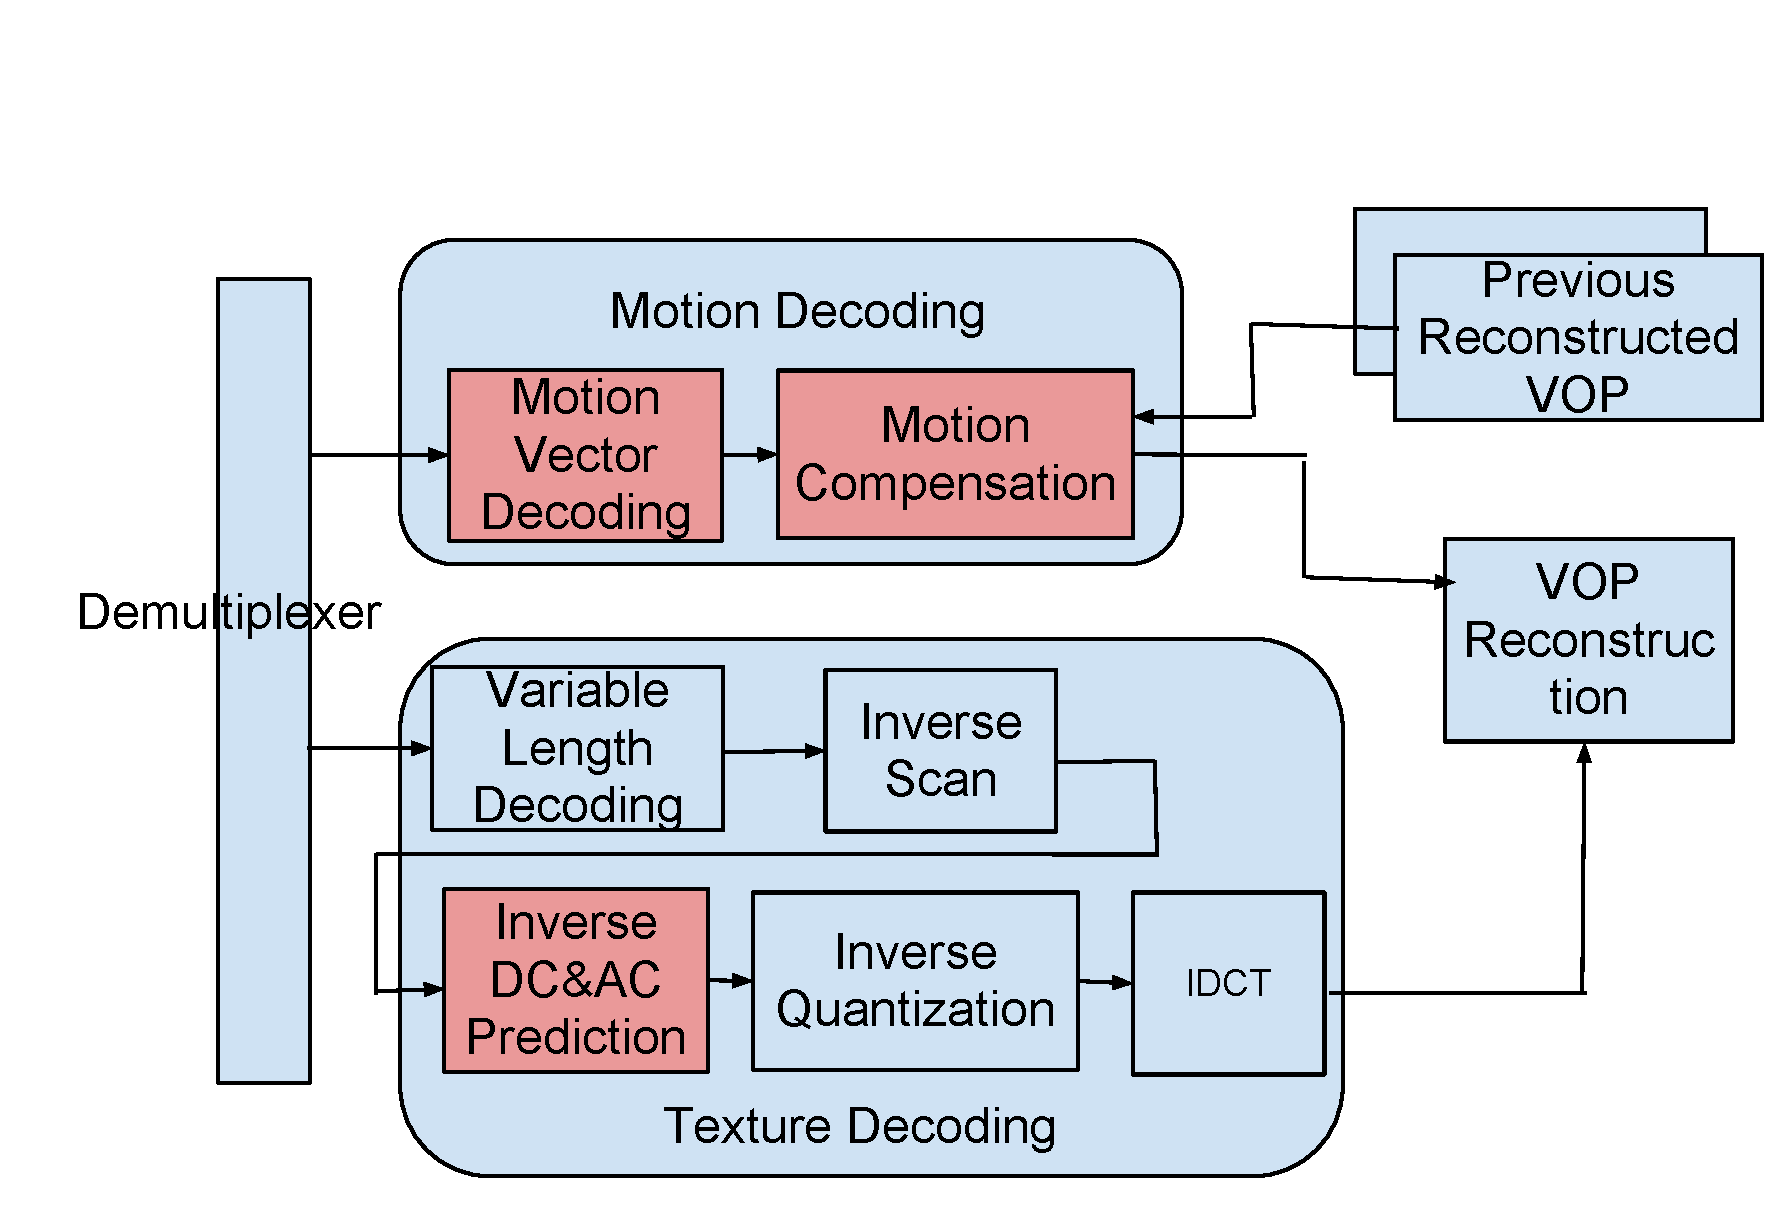
\includegraphics[height=4.5cm]{decoderb.eps}
\caption{A Typical MPEG4 Part 2 Decoder}
\end{figure}
The encoded bitstream is demultiplexed. The coded texture goes through the texture decoding and coded motion is processed by motion decoding. The decoder finally reconstructs the Video Object Plane (VOP). Note that the figure only depicts the core idea of MPEG4 SP decoder, lots of complexities are not covered. 

Various dependencies exist among macroblocks of a MPEG4 SP coded video. From the decoder's pespective, Inverse DC\&AC Prediction phase at Texture Decoding, and Motion Vector (MV) Decoding and Motion Compensation at Motion Decoding of a macroblock are carried out with reference to other macroblocks. Specifically, Inverse DC\&AC Prediction and Motion Vector Decoding are done with reference to other macroblocks in the current VOP, while motion compensation requires macroblocks from previous reconstructed VOP. Because of these dependencies, decoding the MBs of a ROI will require macroblocks outside of ROI to be decoded. 

The selective decoding approach preprocesses the video to obtain the dependencies and save them into files. At decoding, it computes a bitmask based on the dependencies for every VOP on the fly, where the selected macroblocks are marked as '1' and others are marked as '0'. The modified decoder then decodes the selected macroblocks accordingly to the bitmask. In this manner, the macroblocks that are necessary and sufficient to present a clear scene at ROI are decoded. 

In the rest of this paper, section 2 reviews related works. section 3 analyzes the dependencies in detail and discusses the offline computation of selective decoding. Online computation is covered in section 4, including the bitmask generation and modified decoder. Section 5 briefly describes different approaches that validates selective decoding. The proposed approach is implemented in Android platform and described in section 6. We evaluate selective decoding for both video playback frame rate and energy consumption in section 7 and finally conclude at section 8. 





  


  
